\documentclass[a4]{beamer}
\usepackage{amssymb}
\usepackage{graphicx}
\usepackage{subfigure}
\usepackage{newlfont}
\usepackage{amsmath,amsthm,amsfonts}
%\usepackage{beamerthemesplit}
\usepackage{pgf,pgfarrows,pgfnodes,pgfautomata,pgfheaps,pgfshade}
\usepackage{mathptmx}  % Font Family
\usepackage{helvet}   % Font Family
\usepackage{color}

\mode<presentation> {
 \usetheme{Default} % was Frankfurt
 \useinnertheme{rounded}
 \useoutertheme{infolines}
 \usefonttheme{serif}
 %\usecolortheme{wolverine}
% \usecolortheme{rose}
\usefonttheme{structurebold}
}

\setbeamercovered{dynamic}

\title[MA4413]{Statistics for Computing \\ {\normalsize MA4413 Lecture 3A}}
\author[Kevin O'Brien]{Kevin O'Brien \\ {\scriptsize Kevin.obrien@ul.ie}}
\date{Autumn Semester 2013}
\institute[Maths \& Stats]{Dept. of Mathematics \& Statistics, \\ University \textit{of} Limerick}

\renewcommand{\arraystretch}{1.5}

\begin{document}

\begin{frame}
\titlepage
\end{frame}

%---------------------------------------------------------------------------%
\frame{
\frametitle{Today's Class}
\large
\begin{itemize}
\item More on Graphical methods
\begin{itemize}
\item Bar charts
\item Box-and-whisker plots
\end{itemize}
\item Discrete probability distributions
\begin{itemize}
\item Binomial Experiments
\item The Binomial Probability distribution
\end{itemize}
\end{itemize}
}
%------------------------------------------------------------------%
\frame{
\frametitle{Bar plots}
\large
\begin{itemize} \item A bar plot displays the frequency (or relative frequency) for all observations of a discrete random variable. \item A bar plot is much like a histogram, in that the heights of columns represent the frequency (or relative frequency) of each outcome.
\item Each outcome of a random experiment corresponds to one and only one column of the bar plot.
\item A bar plot differs from a histogram in that the columns are distinct and separated from each other by a small distance.
\end{itemize}
}
%------------------------------------------------------------------%
\frame{
\frametitle{Bar plots}
\large
Suppose we roll a die 300 times, and obtain the following results

\begin{center}
\begin{tabular}{|c|c|c|c|c|c|c|}
  \hline

  Outcome & 1 & 2 & 3 & 4 & 5 & 6 \\
  Frequency & 59 &41 &39 &52 &57 &52  \\
  Rel. Freq & 0.196 & 0.136 & 0.130 & 0.173 & 0.190 & 0.173\\
  \hline
\end{tabular}
\end{center}

On the next slide is the bar plot of the relative frequencies of the outcomes of die throw experiment.
Included on the bar plot is the theoretical probability of each outcome. As each outcome is equally probable, this is just a straight line.\\ \bigskip
Minor deviations from the theoretical probability can often be assumed to be as a result of random error. In the case of large deviations, there may be a flawed assumption about the theoretical probabilities.
}

%--------------------------------------------------------%

\frame{
\frametitle{Relative Frequency Bar Plots}

\begin{center}
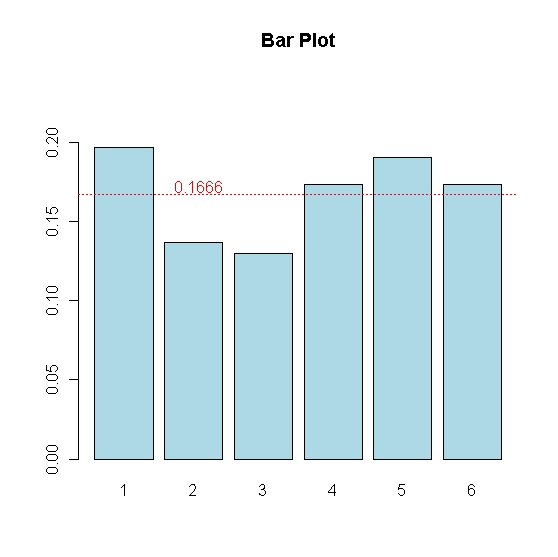
\includegraphics[scale=0.40]{3Bbarplot}
\end{center}
}

%--------------------------------------------------------%

\frame{
\frametitle{Relative Frequency Bar Plots}

\begin{itemize}
\item Just as bar plots can be used to graphically depict observed relative frequencies, they can be used to
depict the theoretical probabilities of each outcome.
\item We will be using bar plots to visualize the theoretical probabilities of outcomes of discrete random variables.
\item For this module, bar plots are assumed to be used for this purpose, unless it is clearly expressed otherwise.
    \item On the next slide is a bar plot of the probabilities of each outcome of a dice throw.
\end{itemize}

}


%--------------------------------------------------------%

\frame{
\frametitle{Bar Plots}
\begin{center}
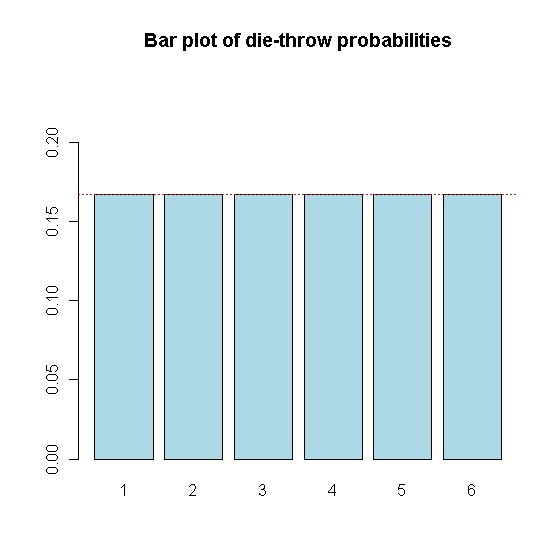
\includegraphics[scale=0.40]{3Bbarplot3}
\end{center}
}

\frame{
\frametitle{Bar Plots}

\begin{itemize}
\item Bar plots are useful in that they visualize `events'.
\item Consider the event where either a `4' or a `5' is thrown.
\item The relevant columns for this event are shaded (next slide).
\item We will be using bar plots for depicting specific events in upcoming material
\end{itemize}

}
%--------------------------------------------------------%

\frame{
\frametitle{Bar Plots}

\begin{center}
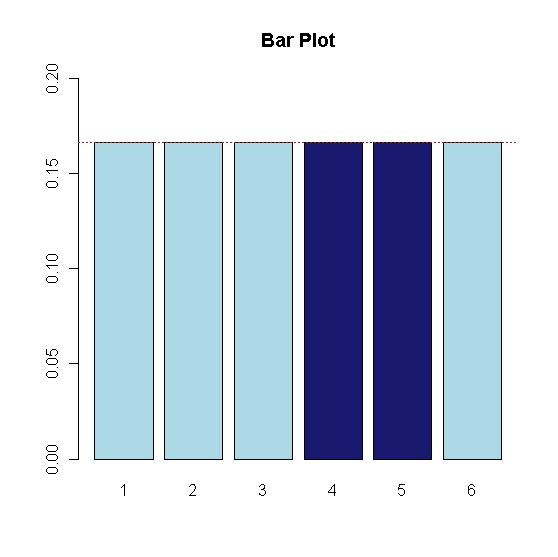
\includegraphics[scale=0.40]{3Bbarplot2}
\end{center}
}


%---------------------------------------------------------------------------%

\frame{
\frametitle{Boxplots}
\begin{itemize}
\item The second graphical method we will be looking at today is the `box-and-whisker' plot (commonly just referred to as `boxplots')
\item The boxplots is a useful tool for assessing the distribution of a dataset, by means of a visual summary.
\item Recall the data set of the exam scores of 100 students from yesterday's class (see next slide).
\item The quartiles of the data set were $Q_1 = 42.5$, $Q_2 = 54.5$ (with $Q_2$ being the median), and $Q_3 =  65.5$ respectively.
\item The interquartile range is $Q_3 - Q_1 = 23$
\item The boxplot of the distribution is featured on the next slide.
\end{itemize}
}
%---------------------------------------------------------------------------%
\frame{
\begin{table}[ht]
\caption{Exam results of 100 students} % title of Table
\centering % used for centering table
\begin{tabular}{|c ccc ccc ccc|} % centered columns (4 columns)\hline
\hline

13	&	21	&	22	&	23	&	24	&	25	&	26	&	28	&	29	&	30	\\	31	&	32	&	33	&	34	&	35	&	 36	&	36	&	36	&	37	&	38	\\
39	&	41	&	41	&	41	&	42	&	43	&	44	&	44	&	44	&	45	\\	45	&	46	&	47	&	49	&	50	&	 51	&	51	&	52	&	53	&	53	\\
53	&	53	&	53	&	54	&	54	&	54	&	54	&	54	&	54	&	54	\\	55	&	55	&	55	&	56	&	56	&	 56	&	57	&	57	&	58	&	59	\\
62	&	63	&	63	&	63	&	63	&	64	&	64	&	64	&	64	&	64	\\	65	&	65	&	65	&	65	&	65	&	 66	&	66	&	66	&	67	&	69	\\
71	&	71	&	72	&	72	&	73	&	74	&	75	&	76	&	76	&	76	\\	77	&	82	&	84	&	85	&	87	&	 88	&	91	&	91	&	92	&	99	\\ \hline
\end{tabular}
\end{table}
}
%--------------------------------------------------------%

\frame{
\frametitle{Boxplots}

\begin{center}
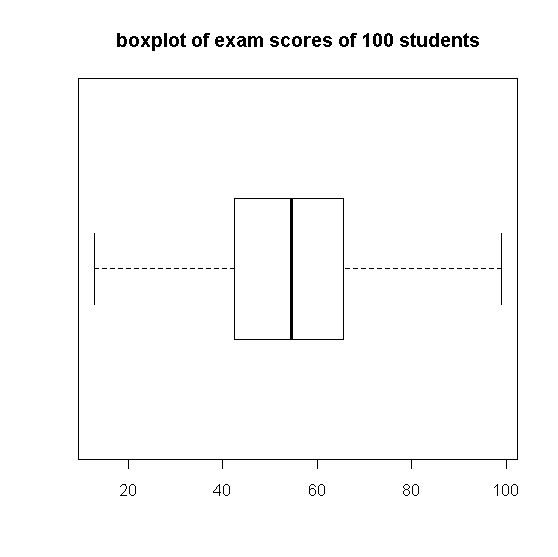
\includegraphics[scale=0.40]{3Bboxplot1}
\end{center}
}


%--------------------------------------------------------------------------------------%
\frame{
\frametitle{Discrete Probability Distributions}

\begin{itemize}

\item Over the next set of lectures, we are now going to look at two important discrete probability distributions

\item The first is the \textbf{\emph{binomial}} probability distribution.

\item The second is the Poisson probability distribution.

\item In \texttt{R}, calculations are performed using the \texttt{binom} family of functions and \texttt{pois} family of functions respectively.
\end{itemize}

}




%-------------------------------------------------------------%
\frame{
\begin{itemize}
\item Now consider an experiment with only two outcomes. Independent repeated trials of such an experiment are
called Bernoulli trials, named after the Swiss mathematician Jacob Bernoulli (1654�1705). \item The term \textbf{\emph{independent
trials}} means that the outcome of any trial does not depend on the previous outcomes (such as tossing a coin).
\item We will call one of the outcomes the ``success" and the other outcome the ``failure".
\end{itemize}
}

%-------------------------------------------------------------%
\frame{
\begin{itemize}
 \item
Let $p$ denote the probability of success in a Bernoulli trial, and so $q = 1 - p$ is the probability of failure.
A binomial experiment consists of a fixed number of Bernoulli trials. \item A binomial experiment with $n$ trials and
probability $p$ of success will be denoted by
\[B(n, p)\]
\end{itemize}
}
%-------------------------------------------------------------%

%---------------------------------------------------------------------------%
\frame{
\frametitle{Probability Mass Function}
\begin{itemize} \item a probability mass function (pmf) is a function that gives the probability that a discrete random variable is exactly equal to some value. \item The probability mass function is often the primary means of defining a discrete probability distribution \end{itemize}
}
%------------------------------------------------------------------%
\frame{
Thirty-eight students took the test. The X-axis shows various intervals of scores (the interval labeled 35 includes any score from 32.5 to 37.5). The Y-axis shows the number of students scoring in the interval or below the interval.

\textbf{\emph{cumulative frequency distribution}}A  can show either the actual frequencies at or below each interval (as shown here) or the percentage of the scores at or below each interval. The plot can be a histogram as shown here or a polygon.
}




\end{document}



%---------------------------------------------------------------------------------------------------------------%
%----R Code ----
%---------------------------------------------------------------------------------------------------------------%
n=60000
Y=numeric(n)
for ( i in 1:n){

X=floor(runif(100,1,7))
Y[i]=sum(X)
}

Y
hist(Y,breaks=seq(300,400,by=10),main=c("Totals of 100 Die Throws"),cex.lab=1.4,font.lab=2,xlab=c("Total Score"))

hist(Y,breaks=seq(300,400,by=20),main=c("Totals of 100 Die Throws"),cex.lab=1.4,font.lab=2,xlab=c("Total Score"))



Z=seq(1:n)
Y/Z

plot(Y/Z,type="l",col="red",main=c("Die Rolls: Running Average"),font.lab=2,ylab="Average Value", xlab=
" Number of Throws")
abline(h=3.5,col="green")


#####################################################

plot(Z,Z.y,pch=16,col="red",ylim=c(2.5,5.5),main=c("Variance"),font.lab=2,ylab=" ", xlab="X: Green  Y: Blue  Z: Red" )

points(Y,Y.y,pch=16,col="blue" )
points(X,X.y,pch=16,col="green" )
points(c(1000,1000,1000),c(3,4,5),pch=18,cex=1.2)
lines(c(1000,1000),c(2.75,5.25),lty=3)



n=100000
Y=numeric(n)
for ( i in 1:n){

X=floor(runif(100,1,7))
Y[i]=mean(X)
}

Y
hist(Y,breaks=seq(270,430,by=2),main=c("Mean of 100 Die Throws (n= 100,000)"),cex.lab=1.4,font.lab=2,xlab=c("Mean of 100 throws")) 